\documentclass[a4paper,10pt]{article}
\usepackage{amsmath,amssymb,graphicx}
\usepackage[hyphens]{url}
\setlength{\emergencystretch}{2em}
\title{Technical Note: Fast Backpropagation for a Finite-Difference Time-Domain Kirchhoff--Carrier String}
\author{Pablo Tablas de Paula, Emmanouil D. Benetos\\ and Joshua D. Reiss\\[0.4em] Centre for Digital Music, Queen Mary University of London}
\date{2026}
\begin{document}
\maketitle
\begin{abstract}
We explain an experimental first-order CUDA adjoint for a nonlinear stiff-string finite-difference time-domain (FDTD) scheme. The underlying update is the non-scalar-auxiliary-variable (non-SAV) Kirchhoff--Carrier reference scheme used by Russo, Ducceschi and Bilbao. A full discrete sine transform retains every grid mode, while a rank-one solve and checkpoint-anchored state reconstruction expose the update and its vector--Jacobian product to a batched GPU kernel. This \emph{Cached adjoint} saves three scalar reductions per step to reduce reconstruction work without treating them as constants in differentiation. We report an existing four-second batch benchmark against naive FDTD autodifferentiation and an upstream modal implementation and state the limits of that comparison.
\end{abstract}

\section{Physical model and reference discretization}
Let $u(x,t)$ denote transverse displacement of a uniform string of length $L$, cross-sectional area $A=\pi r^{2}$, second moment of area $I=\pi r^{4}/4$, density $\rho$, Young's modulus $E$, and tension $T_0$. With $\mu=\rho A$, the damped Kirchhoff--Carrier stiff-string equation is
\begin{equation}
 \mu u_{tt}=T_0u_{xx}-EIu_{xxxx}
 +\frac{EA}{2L}\left(\int_0^L u_x^2\,dx\right)u_{xx}
 -2\mu\sigma_0u_t+2\mu\sigma_1u_{xxt}.
 \label{eq:pde}
\end{equation}
The integral introduces a displacement-dependent tension shared across the string. The benchmark uses simply supported, fixed ends. The conservative nonlinear model and the non-SAV reference update follow the Kirchhoff--Carrier formulation used by Russo et al.\ \cite{russo2026}, which attributes its reference integrator to the conservative Kirchhoff--Carrier scheme of\ \cite[Sec.~8.1.2]{bilbao2009}, with the stiffness and frequency-dependent loss terms discretised as in the explicit stiff-string scheme of the same book (its eq.~7.30a). The damping terms are supported by the accompanying reference code; the validation explicitly enables damping and selects \texttt{SAV=false}. Thus our method differentiates that reference branch, not the alternative SAV algorithm.

With $N$ intervals, spacing $h=L/N$, and timestep $k$, the discretization has $M=N-1$ interior degrees of freedom. For fixed endpoints the complete discrete sine basis diagonalizes both the second and fourth spatial differences. Using all $M$ basis vectors is an invertible change of coordinates for the FDTD grid; it is not a modal truncation. The cached adjoint and the replay adjoint step the state in this basis throughout: the two start states are transformed once, the pickup is read with modal weights, and no spatial transform occurs inside the time loop. The pluck is the raised cosine sampled on the grid nodes and transformed, with an analytic derivative in its centre; the pickup weights are $w_i=\sqrt{2/N}\sin(\pi i x_o)$ for the pickup fraction $x_o$, so both positions have smooth gradients, and the string length enters through $h=L/N$ in the coefficients and the startup step. This distinction matters when comparing with JAX modal synthesis, which uses continuous modal eigenvalues and a different integrator\ \cite{diaz2025}.

The nonlinear part is a rank-one solve. With $u^{n}$ the vector of sine-basis coordinates at step $n$ and $D_{xx}$, $D_{xxxx}$ the diagonalized second and fourth differences, the reference update is
\begin{equation}
 \begin{gathered}
 \mathbf{A}u^{n+1}=\mathbf{B}u^{n}+\mathbf{C}u^{n-1}-q\,\alpha^n,\\
 q=\tfrac{k}{2}\sqrt{hEA/L}\,D_{xx}u^{n},\qquad
 \alpha^n=q^{\mathsf T}\big(u^{n+1}+u^{n-1}\big),
 \end{gathered}
 \label{eq:update}
\end{equation}
with $\mathbf{A}=\mu(1+\sigma_0k)I$, $\mathbf{B}=2\mu I+(T_0k^2+2\mu\sigma_1k)D_{xx}-EIk^2D_{xxxx}$ and $\mathbf{C}=-\mu(1-\sigma_0k)I-2\mu\sigma_1kD_{xx}$, all diagonal in this basis. This is the matrix form of the conservative Kirchhoff--Carrier scheme of\ \cite[eq.~8.11]{bilbao2009} with the stiff-string terms added: up to a constant, $\alpha^n$ is the discrete Kirchhoff--Carrier integral averaged over the two neighbouring time levels, the choice that yields an exact discrete energy balance (eq.~8.9 there). It contains $u^{n+1}$, and the reference solve obtains it first:
\begin{equation}
 \alpha^n=\frac{q^{\mathsf T}u^{n-1}+q^{\mathsf T}\mathbf{A}^{-1}(\mathbf{B}u^{n}+\mathbf{C}u^{n-1})}
                 {1+q^{\mathsf T}\mathbf{A}^{-1}q},\qquad
 u^{n+1}=\mathbf{A}^{-1}\big(\mathbf{B}u^{n}+\mathbf{C}u^{n-1}-q\,\alpha^n\big).
 \label{eq:step}
\end{equation}
This is an algebraic Sherman--Morrison rank-one update\ \cite{sherman1950}. No modes are discarded. The startup states follow the reference implementation and their dependence on physical parameters is also differentiated.

\section{Checkpointed, scalar-cached discrete adjoint}
Reverse-mode differentiation of a loss through a long trajectory ordinarily needs access to intermediate states. Our first-order adjoint saves both state levels every $K$ internal steps. Within each checkpoint segment, it reconstructs the previous state from the later two states and the saved $\alpha^n$ (note that $q$ depends on $u^{n}$ only):
\begin{equation}
 u^{n-1}=\mathbf{C}^{-1}\big(\mathbf{A}u^{n+1}-\mathbf{B}u^{n}+q\,\alpha^n\big).
 \label{eq:inverse}
\end{equation}
The reverse pass then applies the vector--Jacobian product of the complete forward update, accumulates coefficient and initial-state derivatives, and propagates derivatives to density, tension, radius, Young's modulus, length, initial amplitude, $\sigma_0$, $\sigma_1$ and the pluck and pickup positions (fractions of $L$). The pluck position enters through the tangents of the initial states; the pickup is a per-string sine-interpolant readout vector $w(x_o)$, for which the backward kernels also accumulate $\partial\mathcal{L}/\partial w_i=\sum_t\bar y_t\,u_i^t$ per mode, chained through $\partial w/\partial x_o$ by the wrapper. The three saved scalars per step and string are $\alpha^n$, $q^{\mathsf T}q$ and $q^{\mathsf T}(\mathbf{B}u^{n}+\mathbf{C}u^{n-1})$, the inner products behind (\ref{eq:step}). All are already computed during the forward solve. Saving them removes repeated reductions during reconstruction; they are the values needed to evaluate the derivative, \emph{not} constants whose dependencies are ignored. They are also all that the derivative of (\ref{eq:step}) needs: with $a=\mu(1+\sigma_0k)$ and $d=1+q^{\mathsf T}q/a$, the partial derivatives of $\alpha^n$ with respect to $q^{\mathsf T}u^{n-1}$, $q^{\mathsf T}(\mathbf{B}u^{n}+\mathbf{C}u^{n-1})$ and $q^{\mathsf T}q$ are $1/d$, $1/(ad)$ and $-\alpha^n/(ad)$, so $q^{\mathsf T}u^{n-1}$ itself is never formed on the reverse pass. Within a segment the state reconstruction (\ref{eq:inverse}) is independent across modes; the adjoint of $\alpha^n$, $\bar\alpha^n=-q^{\mathsf T}\bar u^{n+1}/a$, is the one quantity that couples them, and the kernel obtains it with a single block reduction per reverse step before accumulating the state and coefficient adjoints per mode. One-scalar reconstruction saves only $\alpha^n$ and recomputes the other two reductions.

For $T$ internal updates, the three-scalar tape costs $3T$ floating-point values per string; the state checkpoints cost approximately $2M(\lceil T/K\rceil+1)$ values. These counts exclude output, loss, gradients, allocator reservations and framework overhead. The three-scalar tape can use more memory than a one-scalar tape, despite being faster in the measured cases. Here $K=256$; the implementation uses float64 and exposes first derivatives only.

One CUDA block handles each string. Threads operate on modes in parallel and exchange the nonlinear coupling through warp and block reductions. Independent strings can run concurrently, but the recurrent time steps and the adjoint propagation remain sequential. Inverse denominators, nonfinite values and checkpoint-boundary reconstruction drift are checked. These checks catch some failures, but passing them does not prove the accuracy of every reconstructed state or gradient. The current experimental CUDA implementation permits at most 256 intervals.

\section{Validation and illustrative measurements}
At matched physical parameters, grid and timestep, a four-second raised-cosine test with 176 intervals and a 132.3\,kHz internal rate compared the CUDA forward result directly with the non-SAV Octave reference. The relative waveform $\ell_2$ difference was $2.45\times10^{-9}$. A separate 2\,ms test compared gradients for all eight physical controls against central finite differences of the Octave output. The normalized mean-square objective's gradients, expressed with respect to relative parameter multipliers, passed a mixed tolerance of $10^{-3}$ relative and $2\times10^{-9}$ absolute. These tests establish agreement for the specified configurations, not convergence to the continuous string over every parameter range.

The timing experiment uses four-second signals, float64, a 44.1\,kHz output, the same loss and eight differentiated physical parameters. The Cached adjoint uses three saved scalars, 176 FDTD intervals (175 discrete modes), a 132.3\,kHz internal rate and antialias filtering. The 175-mode \emph{Modal} comparator uses the genuine upstream \texttt{jaxdiffmodal} solver at a 44.1\,kHz internal rate. Both use the same physical inputs and an initial shape made from eight sine modes, not the raised-cosine test above. The \emph{Autodiff} baseline is a direct PyTorch reverse-mode autodifferentiation of the same FDTD update on the spatial grid (the five-point stencil applied by slicing, the Sherman--Morrison solve written out per step), keeping every intermediate. On a single NVIDIA A100 80\,GB GPU, the medians of three warmed, synchronized evaluations include synthesis, the applicable filtering, loss and backward. Sampled per-process GPU memory includes context and allocator reservations; 10\,ms sampling can miss transient peaks. Compilation and target creation are excluded.

\begin{table}[ht]
\centering
\caption{Four-second forward, loss and backward comparison. Each measured entry is median seconds / sampled GPU GB. HML denotes the 32\,GB host-memory limit; OOM denotes GPU out-of-memory. No timing or GPU-memory value was produced for these cases.}
\label{tab:batch}
\begin{tabular}{rllll}
\hline
Batch & Autodiff & Cached adjoint & Modal & One-scalar \\
\hline
1   & HML & 1.446 / 0.726 & 1.628 / 5.847  & 1.578 / 0.711 \\
2   & HML & 1.462 / 0.851 & 1.542 / 11.484 & 1.584 / 0.833 \\
4   & HML & 1.474 / 1.088 & 1.572 / 19.940 & 1.596 / 1.055 \\
8   & HML & 1.484 / 1.564 & 1.816 / 39.267 & 1.610 / 1.497 \\
16  & OOM & 1.504 / 2.525 & 1.924 / 64.357 & 1.622 / 2.391 \\
32  & OOM & 1.533 / 2.980 & OOM            & 1.650 / 2.710 \\
64  & OOM & 1.583 / 4.167 & OOM            & 1.696 / 3.626 \\
128 & OOM & 2.111 / 6.793 & OOM            & 2.276 / 5.708 \\
\hline
\end{tabular}
\end{table}

At batch 128, the Cached adjoint took 2.111\,s and 6.793\,GB sampled GPU memory; the one-scalar variant took 2.276\,s and 5.708\,GB. Modal ran out of GPU memory at batches 32, 64 and 128. Since this particular initial condition contains only eight modes and the system is unforced, the eight-mode JAX run is also informative: at batch 128 it took 1.451\,s and 35.377\,GB, and its batch-one waveform agreed with the 175-mode JAX waveform to $2.70\times10^{-13}$ relative $\ell_2$. This is an excitation-specific observation, not evidence that eight modes suffice for general plucks.

\begin{figure}[ht]
\centering
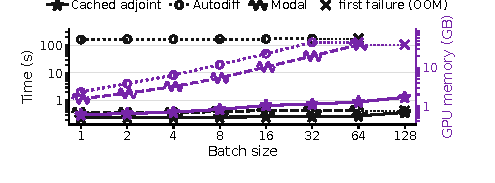
\includegraphics[width=.92\linewidth]{figures/variants/benchmark-main.pdf}
\caption{Four-second batch comparison; black denotes time and purple denotes sampled GPU memory. The Cached adjoint and Modal solvers use distinct integrators and internal rates. Their numerical results do not establish equal physical accuracy.}
\label{fig:comparison}
\end{figure}

For one tested string, the 175-mode JAX waveform and FDTD reference differed by 3.28\% in relative $\ell_2$, while the scaled eight-component gradient vector for the selected loss differed by $1.66\times10^{-5}$ in relative $\ell_2$. The latter is an aggregate, not a per-parameter accuracy bound. Consequently the four-second campaign compared the cost of two stated numerical configurations without establishing equal physical accuracy. Different temporal rates, filters, startup and spatial representations may all matter. The discretization is also not a universal stability or accuracy guarantee across all guitar strings and tunings.

\section{One-second raised-cosine comparison and accuracy}
The one-page abstract now uses a one-second workload with the reference code's raised-cosine pluck (centred at $L/2$, half-width $\lfloor 0.25(N-1)\rfloor$ nodes, i.e.\ $0.244L$ on the 176-interval grid), the same excitation as the Octave validation above. Because the pluck excites every mode, the modal comparator can no longer be run with all 175 grid modes at 44.1\,kHz: for the nominal string only 123 continuous modes lie below 22.05\,kHz, and the exact modal recurrence would alias the rest into the audio band. The abstract's \emph{Modal} therefore uses 100 continuous modes (about 15\,kHz for this string; the count used in Díaz and Sandler's own benchmarks) at 44.1\,kHz.

\texttt{benchmarks/accuracy\_study.py} quantifies the FDTD's own error for the nominal string. The grid is refined along Russo et al.'s path, $h=1.01\sqrt{\gamma}\,h_{\min}(k)$ at $k=1/(44100\cdot\mathrm{OF})$ with $N=2\lfloor L/2h\rfloor$ (the rate is kept an integer multiple of 44.1\,kHz so the project's decimation filter applies; $\gamma$ is the stencil's eigenvalue factor), with the pluck's physical half-width held fixed. With the reference's three-point stencil ($\gamma=1$; OF $=3,6,12,24,48$ gives $N=272,390,556,788,1118$) successive grids differ by factors that follow $(h_{\mathrm{coarse}}/h_{\mathrm{fine}})^2\approx2$, confirming second-order spatial convergence, and the sequence converges to the modal solution: the 123-mode modal waveform is $3.7\times10^{-3}$ from the finest grid in relative $\ell_2$, equal to that grid's own Richardson-estimated distance to the limit. Against that modal solution the former benchmark grid (176 intervals, 3$\times$) was $11.7\%$ away in waveform relative $\ell_2$ over one second, entirely spatial dispersion (raising the oversampling to 6$\times$ left it at $11.9\%$).

\textbf{Fourth-order stencil.} We therefore replace the three-point second difference by the five-point stencil $(-1,16,-30,16,-1)/12h^2$ (the fourth-order five-point stencil with parameter $7/6$ of\ \cite[Sec.~6.3.1]{bilbao2009}; its bound (6.59) gives the $\sqrt3/2$ factor below), closed at the simply supported ends by odd reflection ($u_{-1}=-u_1$), with the fourth difference its square. Every symmetric difference operator with these ends is diagonal in the same discrete sine basis, so the change is a different eigenvalue table, $-4s^2\to-4s^2(1+s^2/3)$ with $s=\sin(\pi n/2N)$: Russo et al.'s time step, the Sherman--Morrison solve, the checkpointing and the CUDA adjoint are unchanged, and the stability bound is the reference's with $h\to h\sqrt{3}/2$ ($\gamma=4/3$). On the 176-interval grid the waveform error against the modal solution drops from $11.7\%$ to $0.45\%$ at 3$\times$ and $1.03\%$ at 2$\times$ (0.18\% at 6$\times$); orders 6 and the exact eigenvalues give the same numbers, so the remainder is the second-order time step. The benchmark uses 176 intervals at 2$\times$ (88.2\,kHz), which is stable over the benchmark's narrow parameter box (every one of the ten parameters within $e^{\pm0.03}$ of the nominal string; corner utilisation 0.93, worst batch item 0.90; $e^{\pm0.05}$ on the material parameters would reach 1.07) though not over the full fitting box, whose corner admits 122 intervals at that rate (152 at 3$\times$). The three-point scheme stays available as \texttt{order=2}; \texttt{test/reference\_paper\_exact.py --order 4} substitutes the five-point operator into the same Octave code so the fourth-order variant is validated against a correspondingly modified reference.
Measured with the implemented stencil (\texttt{benchmarks/accuracy\_study.py --order 4}): the benchmark grid is $1.03\%$ (nominal string) and $1.15\%$ (first benchmark string) from the modal solution in waveform relative $\ell_2$ over one second, $0.51\%$ in FFT magnitude; along the fourth-order refinement path (OF $=3,6,12,24,48$, $N=236,338,480,682,968$) the error against the modal solution falls by a factor of about 2 per level rather than 4, so what remains is first order in the time step, which we attribute to the reference code's startup step (its ``extra $h$ factors''), not to the stencil; the finest grid is $2.5\times10^{-4}$ from the modal solution, whose own truncation (100 vs 123 modes) and time-stepping errors are $1.4\times10^{-5}$ and $3\times10^{-6}$. Against the correspondingly modified Octave reference the five-point scheme matches to $2.0\times10^{-10}$ (CPU) and $5.0\times10^{-10}$ (cached CUDA) relative $\ell_2$ over four seconds at 88.2\,kHz, and its ten gradients, the pluck and pickup positions included, pass the same finite-difference check against the Octave code with its pluck centre and readout made position-dependent, on an off-centre test string ($x_e=0.45L$, $x_o=0.55L$; both position derivatives vanish at the centre by symmetry): the position gradients agree to $1.3\times10^{-7}$ and $8.7\times10^{-8}$ relative, and the largest relative error, $4.3\times10^{-6}$, is on $\sigma_1$, whose gradient is $2\times10^{-6}$ in magnitude (jobs 34846668--34846671).

The one-second timing sweep (\texttt{hpc/native-rate-sweep.sh --loss mae}: Cached adjoint, Autodiff and Modal, batches 1--128, per-case timeout 3600\,s, 32\,GB host limit) is job 34855605 on an A100 80\,GB; its JSON is \url{benchmarks/native_rate_results/a100-sweep-1s-mae-si10-34855605.json}, copied to \url{paper_dmrn2026/figures/} as the figure's data. Each evaluation simulates the batch for one second, forms the mean absolute error of every decimated waveform against the nominal string's (summed over the batch) and backpropagates it to all ten parameters; the batch moves each parameter of each string by up to $\pm3\%$ (\texttt{benchmarks/exact\_methods.py:varied\_material}), and the target keeps the centred pluck and the midpoint pickup. No source file changed during the run; every failure is a CUDA out-of-memory error, and no case timed out or reached the host limit. Table~\ref{tab:sweep} gives the median time per evaluation (forward, loss and ten gradients; three repetitions after warm-up) and the NVML-sampled process GPU memory at the first and the last completed batch. The cached adjoint's time rises by a factor of 1.45 from batch 1 to 128 while its memory grows from 0.6 to 1.5\,GB; Modal is 1.5--1.7 times slower and its memory grows linearly, about 0.6\,GB per batch item, until batch 128 does not fit; Autodiff is about 700 times slower than the cached adjoint, its memory grows by about 1.4\,GB per item, and its host-side autograd graph takes 9.1\,GB of RSS at every batch. Outside the timed region each case is checked against the checkpointed replay (\texttt{replay}, 256-step checkpoints): the cached adjoint's audio and loss are identical to it and its scaled ten-component gradients agree to $3\times10^{-11}$ relative $\ell_2$ at every batch, Autodiff's audio to $4\times10^{-10}$ and its gradients to $1.5\times10^{-9}$; Modal's first item is $9.6\times10^{-3}$ from the FDTD waveform ($5.6\times10^{-3}$ in FFT magnitude) with scaled gradients $1.3\times10^{-4}$ apart, consistent with the accuracy study above. The earlier sweep with the six perceptual controls perturbed, eight gradients and the STFT cumulative-energy loss (job 34614181) gave the same picture (0.245--0.371\,s, 0.373--0.424\,s and 162--174\,s for the three methods) and stays archived beside it.

\begin{table}[ht]
\centering\small
\begin{tabular}{llll}
\hline
Method & batch 1 & last completed batch & first failure \\
\hline
Cached adjoint & 0.240\,s, 0.57\,GB & 128: 0.348\,s, 1.51\,GB & none \\
Modal (100 modes) & 0.377\,s, 1.53\,GB & 64: 0.419\,s, 39.3\,GB & 128 (GPU OOM) \\
Autodiff & 169\,s, 2.33\,GB & 32: 177\,s, 44.9\,GB & 64 (GPU OOM) \\
\hline
\end{tabular}
\caption{One-second sweep, job 34855605 (ten parameters, MAE loss, $\pm3\%$ batch): median seconds per evaluation and sampled GPU memory at the first and last completed batch.}
\label{tab:sweep}
\end{table}

\textbf{Checkpointed baselines.} A reviewer of the abstract noted that both baselines run as distributed, without rematerialisation, so their linear memory growth confounds the comparison of methods with an implementation choice. Two variants isolate that choice, everything else unchanged (jobs 35062741 and 35105080, the same GPU model; \texttt{benchmarks/native\_rate\_results/a100-ckpt*-35062741.json}, \texttt{a100-ckptro-*-35105080.json}, merged with the original sweep by \texttt{paper\_dmrn2026/figures/merge\_sweeps.py}). \emph{Autodiff, checkpointed} cuts the spatial PyTorch loop into 256-step chunks and passes each through \texttt{torch.utils.checkpoint} (non-reentrant form), the same segments as the cached adjoint's checkpoints; its values and ten gradients equal the plain path bit for bit (\texttt{test/figure\_fdtd.py}) and its gradients agree with the replay adjoint to $1.5\times10^{-9}$ at every batch. \emph{Modal, checkpointed} rewrites the upstream \texttt{solve\_tf} recurrence (its coefficients, RK4 first step and two-term update) as a \texttt{jax.lax.scan} over 256-step segments whose body is wrapped in \texttt{jax.checkpoint}, the package itself untouched; values and gradients match upstream to $10^{-13}$ and $10^{-10}$ (\texttt{test/native\_rate\_study.py}). Returning the full modal trajectory and its velocities as the upstream interface does still costs two (steps, modes) arrays per item and their cotangents, 0.2\,GB per batch item (0.99 to 26.5\,GB over batches 1 to 128, a third of the plain variant), so the variant in the abstract's figure also reads the pickup inside the scan, as the FDTD kernels do, and returns the waveform only; its waveform is identical to the plain modal solver's. Table~\ref{tab:ckpt} gives the result: checkpointing brings both baselines to the cached adjoint's memory, every batch fits, and the time rises by a factor of 1.5 (Autodiff) and 1.3 to 1.5 (Modal), the price of recomputing each segment's forward pass. The cached adjoint remains 760 to 1070 times faster than checkpointed autodiff and 1.7 to 2.1 times faster than the checkpointed modal solver at matched memory: the flat memory is a property of checkpointing that the baselines share once they use it, the speed is the kernel's.

\begin{table}[ht]
\centering\small
\begin{tabular}{llll}
\hline
Method & batch 1 & batch 128 & first failure \\
\hline
Cached adjoint (job 34855605) & 0.240\,s, 0.57\,GB & 0.348\,s, 1.51\,GB & none \\
Autodiff, checkpointed & 256\,s, 0.57\,GB & 264\,s, 1.80\,GB & none \\
Modal (100), checkpointed, trajectory returned & 0.479\,s, 0.99\,GB & 0.615\,s, 26.5\,GB & none \\
Modal (100), checkpointed, readout in scan & 0.497\,s, 0.99\,GB & 0.606\,s, 1.27\,GB & none \\
\hline
\end{tabular}
\caption{One-second sweep of the rematerialised baselines (ten parameters, MAE loss, $\pm3\%$ batch, A100 80\,GB): median seconds per evaluation and sampled GPU memory at the first and last batch. Plain Autodiff and Modal ran out of memory at batches 64 and 128 (Table~\ref{tab:sweep}).}
\label{tab:ckpt}
\end{table}

\bibliographystyle{plain}
\bibliography{references}
\end{document}
